
Many high energy experiments require pure electron beams. Despite the steady improvement of the beam lines,
contamination below a level of few \% is very difficult to achieve. An example is the NA64 experiment\cite{na64} at CERN
in which it is mandatory to suppress hadron and muon contamination in the electron beam since such particles can
generate irreducible background processes mimicking the experimental signature of a dark photon \cite{prlpaper, proposal}.
NA64 uses 100 GeV electrons from beam lines provided by the Super Proton Synchrotron (SPS) at CERN which is one of the
best existing beam lines at this energy in terms of beam purity\cite{sps}.\par

Since the electrons are secondary particles from the proton beam at the SPS, the experiment uses magnets to remove the
remaining hadrons (pions and kaons) and some low-energy electrons from the interaction with passive material along the
beam line. For this reason, the experiment use the synchrotron radiation to tag the incoming electrons and reject the
other events.\par

In this chapter we start by briefly describing the NA64 experiment goals and the advantage of it. The experiment has two
different configuration for two possible dark photon decays, {\it visible} and {\it invisible}. These two configurations are
discussed, however, the focus is on the {\it invisible decays} setup, where results are shown.\par

To detect a dark photon signal a pure electron beam must be achieve how the dark photon signal can be detected. Then we
discuss about the three different options of synchrotron radiation detector (SRD) presents for the experiment and we
focus on of them, the LYSO crystals array. We present the experimental results of the hadron suppression level and we
compare with the first option for SRD a BGO crystals array. Finally, we present the published results from the NA64
experiment searching for dark missing energy events of dark photons.\par


\section{NA64 experiment}

The NA64 experiment is a fixed-target experiment at the CERN SPS combining the active beam dump and missing energy
techniques to search for rare events.\par

A fully hermetic detector placed on the H4 beam line has been built with the primary goal to search for light dark
bosons ($Z'$) from dark sector that are coupled to photons, e.g. dark photons ($A'$), or sub-GeV $Z'$ coupled only to
quarks. In some cases the $Z'$ is coupled only to $\mu$ or $\tau$, so we call the $Z'$ the dark leptonic gauge boson.
The experiment is also capable to search for $K_L \rightarrow ${\it invisible} decay, which is complementary to
$K^+\rightarrow \pi^+ + \nu \nu$, and invisible decays of $\pi_0$, $\eta$, $\eta'$, $K_S$ mesons.\par

The advantage of this approach is that the sensitivity (or number of signal events) of the experiment is roughly
proportional to the $Z'$ coupling squared $\varepsilon^2$, associated with the $Z'$ production in the primary interaction
in the target, while in a classical beam dump experiment, it is proportional to $\varepsilon^4$, one $\varepsilon^2$
came from the $Z'$ production, and another $\varepsilon^2$ is either from the probability of $Z'$ decays or their
interactions in a detector located at a large distance from the beam dump.\par

The sensitivities of these two methods depend on the region under study in the ($\varepsilon^2$,$m_Z$) parameter space,
background level for a articular process, available beam intensity (Figure \ref{fig:prodrate}), etc.\par

In some cases, much less running time and primary beam intensity are required to observe a signal event with our
approach.\par


\begin{figure}[ht]
	\hspace*{\fill}
	\centering
	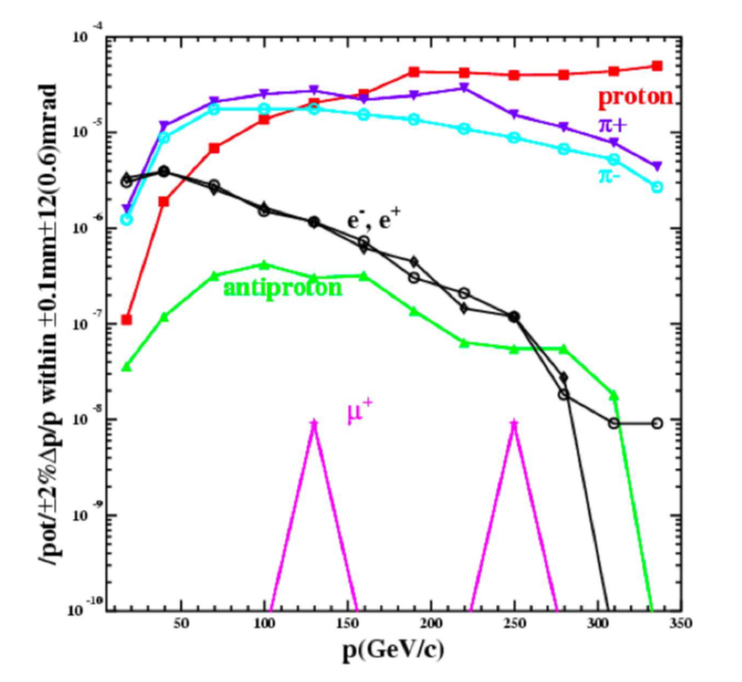
\includegraphics[width=0.5\textwidth]{productionrate.png}
	\hspace*{\fill}
	\caption{Beam intensity of H4 beam line from target T2 at SPS, CERN.}
	\label{fig:prodrate}
\end{figure}

One of the main background sources in the experiment is related to the possible presence of the low-energy tail in the
energy distribution of beam electrons. This tail was observed during irradiation of the setup by the \SI{100}{GeV}
electron beam without switching on the deflecting magnet\textcolor{red}{electron tail}. This tail is caused by the
electron interactions with a passive material, e.g. as entrance windows of the beam lines, residual gas, etc... Another
source of low energy electrons is due to the pion or muon decays in flight in the beam line. The uncertainties arising
from the lack of knowledge of the dead material composition in the beam line are potentially the largest source of
systematic uncertainty in accurate calculations of the fraction and energy distribution of these events. Hence, the
sensitivity of the experiment could be determined by the presence of such electrons in the beam, unless one takes
special measures to suppress this background. To reject these background sources at high energies by using standard
techniques,e.g. threshold Cerenkov counters, is practically impossible.\par

To improve the high energy electrons selections and suppress background from the possible admixture of low energy
electrons, we use a tagging system utilizing the synchrotron radiation (SR) from high energy electrons in a dipole
magnet, installed upstream of the detector. The basic idea is that, since the critical SR photon energy is $(\hbar
\omega)_{\gamma}^c \propto E_0^3$, the low energy electrons in the beam could be rejected by using the cut, e.g.
$E_{\gamma}>0.3(\hbar\omega)_{\gamma}^c$, on the energy deposited in the SR detector. 



\subsection{Physics Motivation}

\begin{equation}
{\cal L} = {\cal
L}_{SM}-\frac{1}{4}F'_{\mu\nu}F'^{\mu\nu}+\frac{\epsilon}{2}F'_{\mu\nu}F^{\mu\nu}+\frac{m^2_{A'}}{2}A_{\mu}'A'^{\mu}+i\bar{\chi}\gamma^{\mu}\partial_{\mu}\chi-m_{\chi}\bar{\chi}\chi-e_D\bar{\chi}\gamma^{\mu}A'_{\mu}\chi
\end{equation}
Standard Model.\\
$g_{\mu}-2$ muon anomaly\\
 


\subsection{Dark Photon signal}

U(1) broken symmetry $\longrightarrow$ massive dark photon\\
type of mixing
coupling constant and sub-GeV mass connect with g2 muon anomaly.
How to detect him?
\subsubsection{Visible decay}


\begin{figure}[ht]
	\hspace*{\fill}
	\centering
	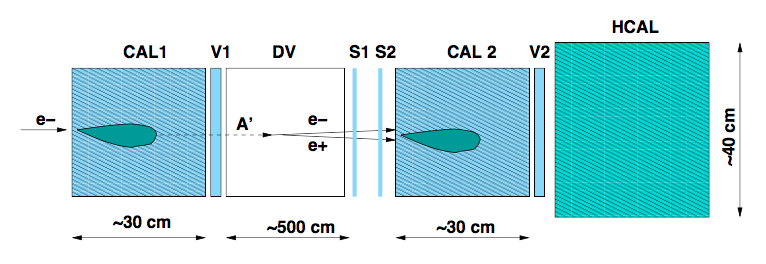
\includegraphics[width=0.5\textwidth]{schemevis.png}
	\hspace*{\fill}
	\caption{}
	\label{fig:schemevis}
\end{figure}

\begin{equation}
\mathrm{S_{A'} = CAL1 \cdot \overline{V1}\cdot S1\cdot S2\cdot CAL2\cdot \overline{V2}\cdot\overline{HCAL}}
\end{equation}

\begin{figure}[ht]
	\hspace*{\fill}
	\centering
	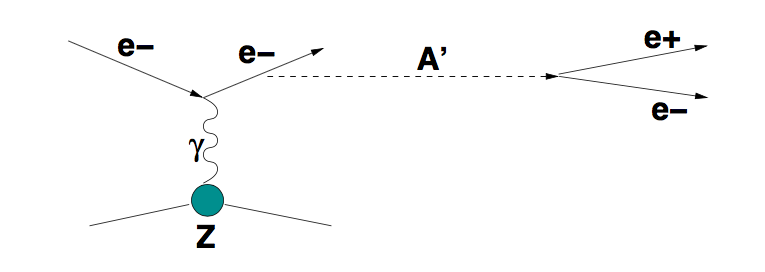
\includegraphics[width=0.5\textwidth]{visible.png}
	\hspace*{\fill}
	\caption{Diagram illustrating the massive $A'$ production in the reaction $e^-Z\rightarrow e^-ZA'$ of electrons
	scattering off a nuclei ($A$, $Z$) with the subsequent $A'$ into an $e^+e^-$ pair.}\label{fig:vis}
\end{figure}


\subsubsection{Invisible decay}
\begin{figure}[ht]
	\hspace*{\fill}
	\centering
	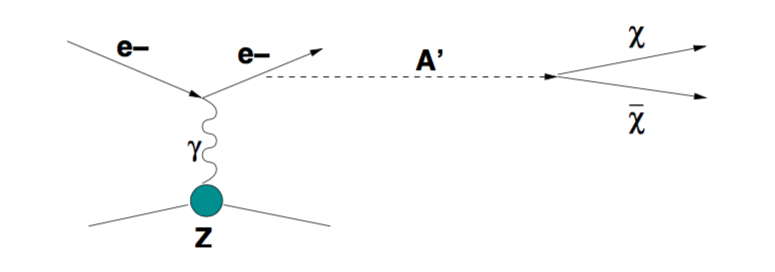
\includegraphics[width=0.5\textwidth]{invisible.png}
	\hspace*{\fill}
	\caption{Production rate at H4 beam line}\label{fig:inv}
\end{figure}

\begin{figure}[ht]
	\hspace*{\fill}
	\centering
	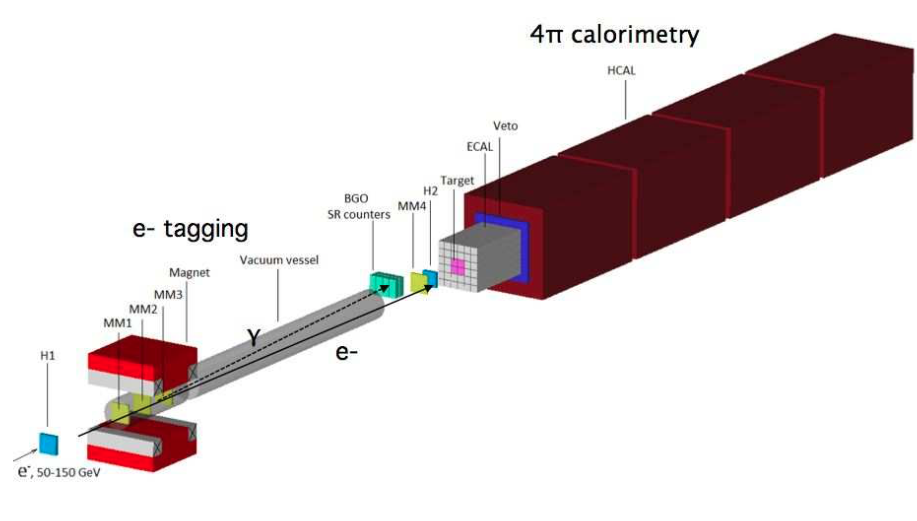
\includegraphics[width=0.8\textwidth]{schemeinv2.png}
	\hspace*{\fill}
	\caption{}\label{fig:schemeinv}
\end{figure}

The method of the search is the following. The incident electron energy absorption in the ECAL is accompanied by the
emission of bremsstrahlung $A'$s in the reaction $eZ\rightarrow eZA'$ of electrons scattering on nuclei, due to the
$\gamma - A'$ mixing. The diagram for the $A'$ production in the reaction is shown in \ref{fig:inv}.\par

The reaction typically occurs in the first few radiation length ($X_0$) of the calorimeter. The part of the primary beam
energy is deposited in the ECAL, while the remaining fraction of the total energy is transmitted by light dark matter
decay particles $\chi$ through the rest of the detector. The $\chi$ penetrates the ECAL, veto V and the HCAL without
interactions resulting in the missing-energy signature in the detector.\par

The occurrence of $A'\rightarrow invisible$ decays produced in $e^-Z$ interactions would appear as an excess of events
with a single electromagnetic shower in the ECAL1,Fig. \ref{fig:schemeinv}, and zero energy deposition in the rest of
the detector (V and HCAL), above those expected from the background sources. The signal candidate events have the
signature:\par



\begin{equation}
\mathrm{ S_{A'} = H1 \cdot H2\cdot ECAL (E_{ECAL}<E_0)\cdot \overline{V\cdot HCAL}}
\end{equation}
and should satisfy the following selection criteria:
\begin{itemize}
\item The momentum of the incoming particle track should correspond to the beam momentum.
\item The starting point of (e-m) showers in the ECAL should be localized within a few first $X_0$s.
\item The lateral and longitudinal shapes of the shower in the ECAL are consistent with an electromagnetic one. The
fraction of the total energy deposition in the ECAL is $f<0.5$.
\item No energy deposition in the V and HCAL.
\end{itemize}

To improve the primary high energy electrons selection and additionally suppress background from the possible presence
of low energy electrons in the beam typically with energy $E_e <0.5 E_0$ (see below), one use a high energy $e^-$ tagging
system utilizing the synchrotron radiation (SR) from high energy electrons in a dipole magnet, as schematically shown in
Fig. \ref{fig:schemeinv}. 




\subsection{Detector}

The $A'$ production is a rare event. For the interesting parameter range it is expected to occur with a rate $10^{-9}$
with respect to the ordinary photon production rate. Hence, its observation represents a challenge for the detector
design and performance.\par

The experimental setup specifically designed to search for the $A'$ production in the reaction (4) of high-energy
electron scattering off nuclei in a high density target T is schematically shown in Fig. 3. The experiment employs the
upgraded H4 electron beam line at the CERN SPS described in details in \textcolor{red}{Ref.[21]}. The beam is designed
to transport the electrons with the maximal intensity $\simeq (3-4) \cdot 10^6$ per SPS spill in the momentum range
between \SIrange{50}{150}{GeV/c} that could be produced by the primary proton beam of \SI{450}{GeV/c} with the intensity
up to a few $10^{12}$ protons on target. The electrons are produced by protons impinging on a primary beryllium target and
transported to the detector inside the evacuated beam-line tuned to an adjustable beam momentum. \par

The hadron contamination in the electron beam is $\pi/e < 10^{-2}$ and the size of the beam at the detector position is
of the order of a few \si{\square\centi\metre}.

The detector shown in Fig. 3 utilizes upstream magnetic spectrometers (MS) consisting of dipole magnets and a
low-material-budget tracker, which is a set of Micromegas chambers , MM1-MM4, allowing the reconstruction and precise
measurements of momenta for incident electrons \cite{mm}. It also uses the scintillating counters S0, S1 and hodoscopes H1
and H2 to define the primary beam, and the active target T, which is the central part of the high-efficiency hodoscopic
electromagnetic calorimeter (ECAL) used for the accurate measurement of the recoil electron energy from the reaction
(4). Downstream the target the detector is equipped with high-efficiency forward veto counter V, and a massive,
completely hermetic hadronic calorimeter (HCAL). Three straw-tubes chambers, MUON1-MUON3, located between the HCAL
modules are used for the final-state muon(s) identification. The modules serve as a dump to completely absorb and detect
the energy of hadronic secondaries produced in the electron interactions $e^-A\rightarrow anything$ in the target. In
order to suppress backgrounds caused by the detection inefficiency the HCAL must be longitudinally completely hermetic
[18, 19]. To enhance its hermeticity, the HCAL thickness is chosen to be $\simeq  30 \lambda_{\mathrm{int}}$ (nuclear
interaction lengths). The 15 m long vacuum vessel between the magnet and the ECAL is installed to avoid absorption of
the synchrotron radiation photons detected at the downstream end of the vessel by the array of BGO crystals for the
effective tagging of the incoming beam electrons [18].





\begin{figure}[ht]
		\hspace*{\fill}
		\centering
		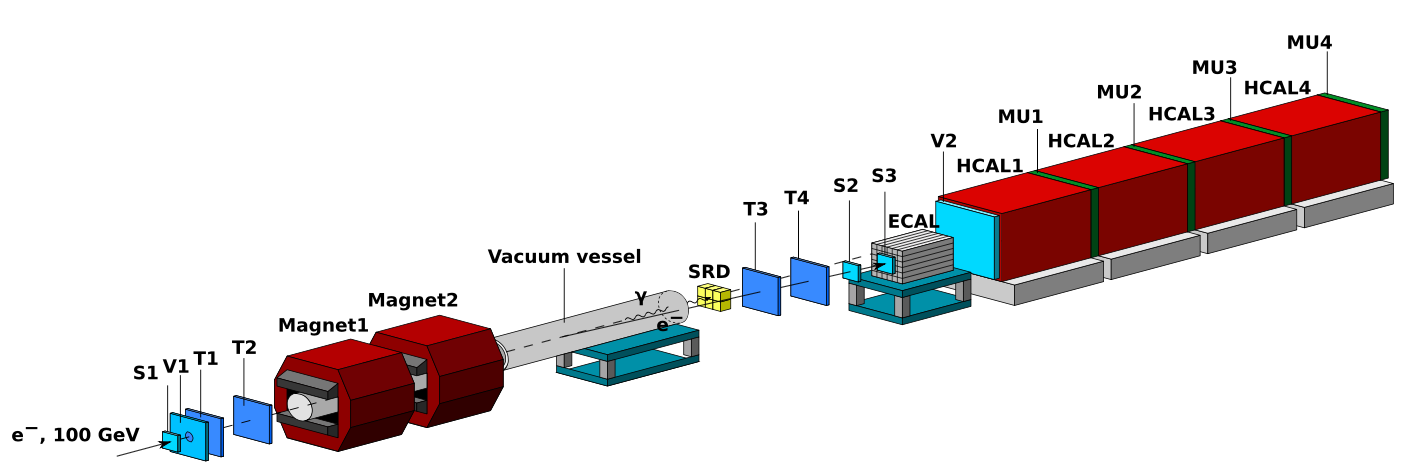
\includegraphics[width=\textwidth]{na64detector.png}
		\caption{Schematic illustration of the setup to search for $A'\rightarrow${\it invisible} decays with 100GeV e$^-$
		at H4 beam line. the incident electron energy absorption in the ECAL is accompanied by the emission of
		{\it bremsstrahlung} $A'$s in the reaction $eZ\rightarrow eZA'$ of electron scattering on nuclei, see Diagram
		interaction. The part of the primary beam energy is deposited in the ECAL, while the remaining fraction of the total
		energy is transmitted by the decay dark matter particles through the rest of the detector resulting in the missing
		energy signature in the detector.}\label{fig:na64detector}
\end{figure}

\subsection{Particle identification}

The hadron contamination in the electron beam lead us to idifentify the particle before it reaches the active target
(ECAL). For particle identification in high energy physics is commonly used detection of Cherenkov radiation. This type
of electromangetic radiation is emitted when a charged particle passes trhough a dielectric medium at a speed ($v$) greater
than the phase velocity of light ($c/n$) in that medium. Hence the condition to emmitt Cherenkov radiation is when
\begin{equation}\label{condCR}
\frac{v}{c} = \beta > \frac{1}{n} 
\end{equation}
where $n$ is the refraction index of the medium. 

The equation \ref{CRemission} represent the energy radiated as Cherenkov radiation per frequency and per unit distance along the path of
the particle. \par
In this experiment the dielectric medium is the air with an refraction index of $n_{air}=1.0002772$. Therefore for an
specific frequency $\omega_0$ is possible to estimate the amount of photons emmited by an electron or a pion. 

\begin{equation}\label{CRemission}
\left(\frac{d^2E}{dxd\omega}\right)_{rad} = \frac{\omega q^2}{c^2}
\left(1-\frac{1}{\beta^2\epsilon(\omega)}\right) 
\end{equation}
where $q$ is the charge, $\beta$ the velocity of the particle and $\epsilon(\omega)$ is the electrical permitivity of the medium 


\begin{


%------------------- SYNCHROTRON RADIATION ------------------


\section{Synchrotron Radiation Detector}


A charged particle in a magnetic field moves in a circular motion emitting photons along its trajectory due to the basic
principles of electrodynamics. Both quantum and classical theory of synchrotron radiation (SR) are well understood
\ref{}. In the range of interest for our experiment both treatments are equivalent and we can therefore use the
classical approximation for our calculations. The total power $S$ emitted per unit length by a relativistic charged
particle of energy $E$ with mass $M$ and with bending radius $R$ in a magnetic field $B$ perpendicular to its velocity
is given by:


\begin{equation}
S = \frac{q^2c}{6\pi}\frac{1}{(Mc^2)^4}\frac{E^4}{R^2}
\end{equation}

where $q$ is the charge of the particle and $c$ the speed of light. Since the emission angle of the synchrotron is
proportional to the inverse of the Lorentz factor $\gamma$, the photons are emitted tangentially to the particle
trajectory.\par

Hence under a circular acceleration, an charged particle, e.g. an electron, emits synchrotron radiation and the energy radiated per
particle per turn being

\begin{equation}
\Delta E = \frac{e^2\beta^3}{3\varepsilon_0 R}\left (\frac{E}{mc^2}\right )^4
\end{equation}
Putting the numerical values for $\varepsilon_0$ and $e$, and setting $\beta=1$

\begin{equation}
\Delta E = 0.08856\frac{E^4}{R}
\end{equation}

where $\Delta E$ is in \unit{MeV}, $E$ is in \unit{GeV} and $R$ is in meters. Thus for relativistic $\pi^-$'s and
$e^-$'s of the same energy, the energy loss is $(m_e/m_{\pi^{\pm}})^4\sim 10^{-10}$ times less for a $\pi^{\pm}$. This
would be the case if the particles propagate in an ideal vacuum. However, in a real experimental setup, vacuum windows,
residual gas, beam counters such as scintillators and trackers result in interactions of the incoming particles with
material. Therefore, the suppression factor when crossing materials is limited by the emission of secondary electrons
with enough kinetic energy (several MeV) to leave a synchrotron-like signal in the detector. Although most of the energy
transfer due to ionization for heavy charged particles is only a few keV, rare high energy transfer is possible. The
distribution of such secondary electrons with kinetic energy $T>>I$, where $I$ is the mean excitation energy of the
atom/molecule, for a particle with velocity $\beta$ and charge $z$ passing through a material with atomic number $Z$,
mass number $A$ and thickness $dx$ is described by \textcolor{red}{ref}:

\begin{equation}
\frac{d^2N}{dTdx}=\frac{1}{2}Kz^2\frac{Z}{A}\frac{1}{\beta^2}\frac{F(T)}{T^2}
\end{equation}

The constant $K$ is defined as $K=4\pi N_A r^2_em_ec^2$ where $N_A$ is the Avogadro's number, $r_e$ is the classical
electron radius and $m_e$ the electron mass. $F(T)$ is a spin-dependent factor, which in our case for $T<<W_{max}$ is
very close to unity. $W_{max}$ is the maximal energy transfer in a single collision to the electron:

For a $\pi^-ZZ$ at \si{\giga\electronvolt}, $W_{max}$ is roughly 1\si{\giga\electronvolt} which covers completely the
energy range where synchrotron radiation is emitted. 


\begin{figure}[ht]
	\hspace*{\fill}
	\centering
	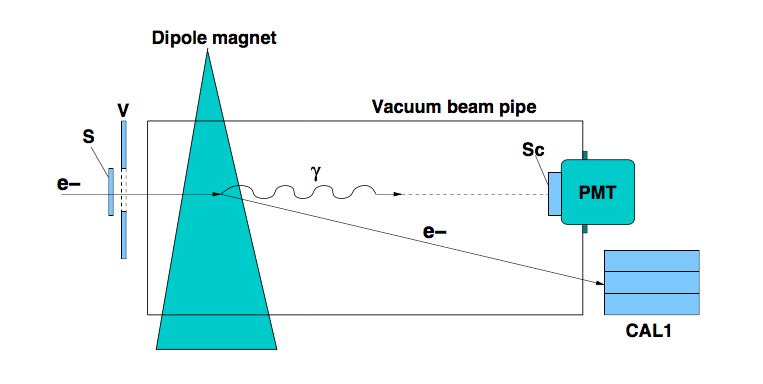
\includegraphics[width=0.8\textwidth]{schemeinv.png}
	\hspace*{\fill}
	\caption{The scheme of the additional tagging of high energy electrons in the beam by using the electron synchrotron
	radiation in the bending magnetic dipole. The synchrotron radiation photons are detected by a $\gamma$-detector by
	using scintillator as BGO crystals, LYSO crystals or different configuration with Pb+Sc. All theses options are viewed
	by a high quantum efficiency PMT or SiPM. The beam defining counters are also shown.}
	\label{fig:schemeinv}
\end{figure}
\begin{figure}[ht]
	\hspace*{\fill}
	\centering
	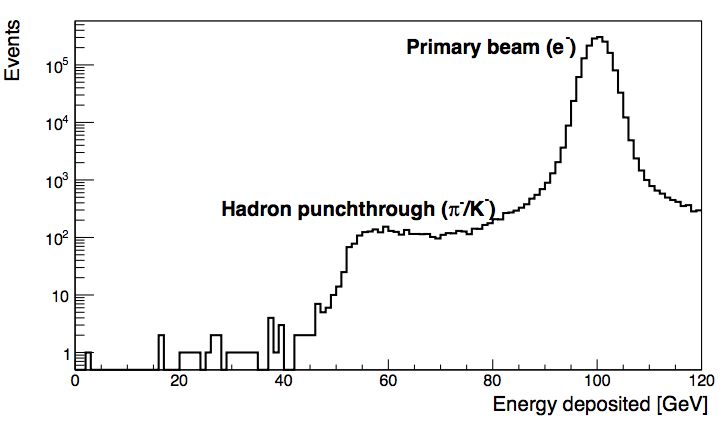
\includegraphics[width=0.8\textwidth]{ecalspectra.png}
	\hspace*{\fill}
	\caption{}\label{ecalspectra}
\end{figure}

%----------------------------- BGO ----------------------------- 
\subsection{BGO}\label{bgoanal}

The idea to use scintillator crystals as synchrotron radiation detector for tagging electrons has been tested
before\cite{bgosync}. However, this time the idea is to reject hadrons to the level of $10^{-5}$ compare to the
electrons on target. The NA64 experiment, use as a first option of SRD an array of $\mathrm{Bi_4Ge_3O_{12}}$ (BGO)
crystals because of its high photoelectric gamma rays absortion and a configuration that can the dectect the incoming SR and reject
the back scattering event coming from the ECAL.\par
The detector consists of 8 hexagonal crystals with an external diameter of \SI{55}{mm} and a length of
\SI{200}{mm}. The crystals are grouped into two modules. Each crystal is wrapped in Teflon tape for efficient light
collection and it is glued to an ETL 9954 photomultipliers(PMT).\par

The BGO has a density of 7.13 \si{\gram/\centi\cubic\metre} and because of the high atomic number of the bismuth
component ($Z=83$) it has one of the larges probability per unit volume for photoelectric absorption of gamma rays.
\cite{bgodatashet}. The light yield of about 8500 $\gamma$s/MeV coupled to the transportation losses and
quantum efficiency of the PMT gives an energy resolution of about 17\% (FWHM) at \SI{1.27}{MeV} (measured with a
$\mathrm{^{22}Na}$ radioactive source).\par




\begin{figure}[ht]
		\centering
		\hspace*{\fill}
		\begin{subfigure}[b]{0.45\textwidth}
			\centering
			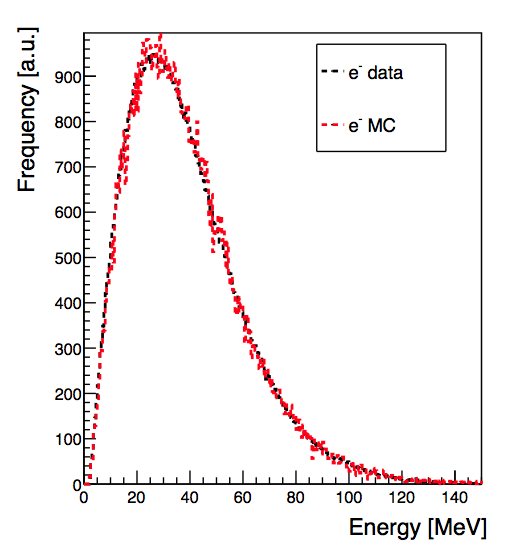
\includegraphics[width=\textwidth]{bgoe.png}
			\caption{}\label{}
		\end{subfigure}
		\hfill
		\begin{subfigure}[b]{0.45\textwidth}
			\centering
			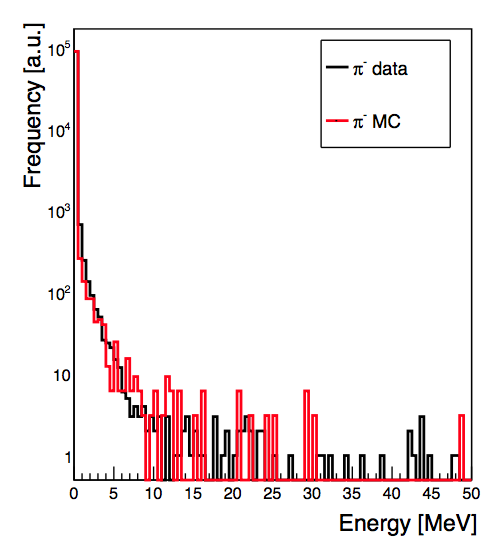
\includegraphics[width=\textwidth]{bgopi.png}
			\caption{}\label{}
		\end{subfigure}
		\hspace*{\fill}
		\caption{}\label{}
\end{figure}
\begin{figure}[ht]
		\centering
		\hspace*{\fill}
		\begin{subfigure}[b]{0.45\textwidth}
			\centering
			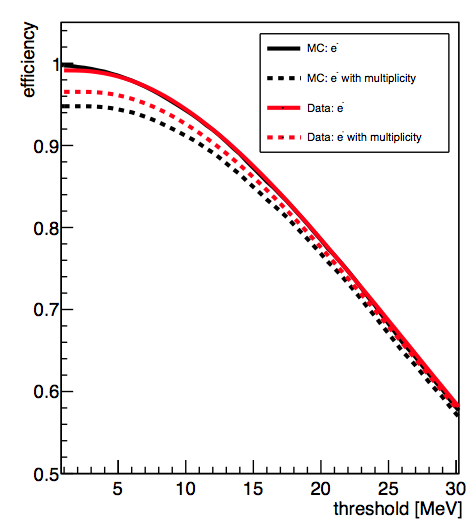
\includegraphics[width=\textwidth]{bgoeff.png}
			\caption{}\label{}
		\end{subfigure}
		\hfill
		\begin{subfigure}[b]{0.45\textwidth}
			\centering
			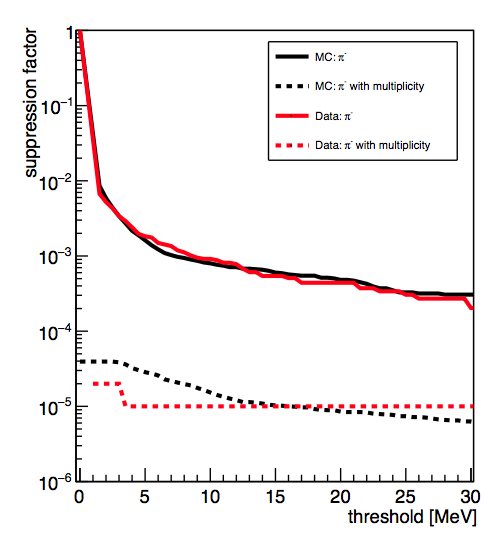
\includegraphics[width=\textwidth]{bgosup.png}
			\caption{}\label{}
		\end{subfigure}
		\hspace*{\fill}
		\caption{}\label{}
\end{figure}


%----------------------------- LYSO  ----------------------------- 
\subsection{LYSO}

The setup for invisible decays has a second option of scintillating material to detect synchrotron radiation. An array
of LYSO\cite{lysogobain} crystals with a shorter time decay and fourth time light output compare to BGO.
An array of 25x25 crystals of 4x4x45\si{\cubic\milli\metre} has been build at the Technical
University Federico Santa Maria. Each crystal is a Cerium doped lutetium ($\mathrm{Lu_{1.8}Y_{0.2}SiO_5:Ce}$), with a
light output of 35.000 [photons/MeV]. This type of crystals has a short time decay (see Table \ref{property}) compared
to BGO crystals.  Therefore, it is a more suitable candidate for a SR detection at high rates. With a decay time of
$\mathrm{\tau_{LYSO}=40}$ns, allows to a maximal electron counting rate of $\lesssim 1/\tau \sim 10^7 e^-/s$.\par

The light is collected from KURARAY wave length shifter (WLS) fibers 

\subsubsection{Readout}
\begin{figure}[t]
	\hspace*{\fill}
	\centering
	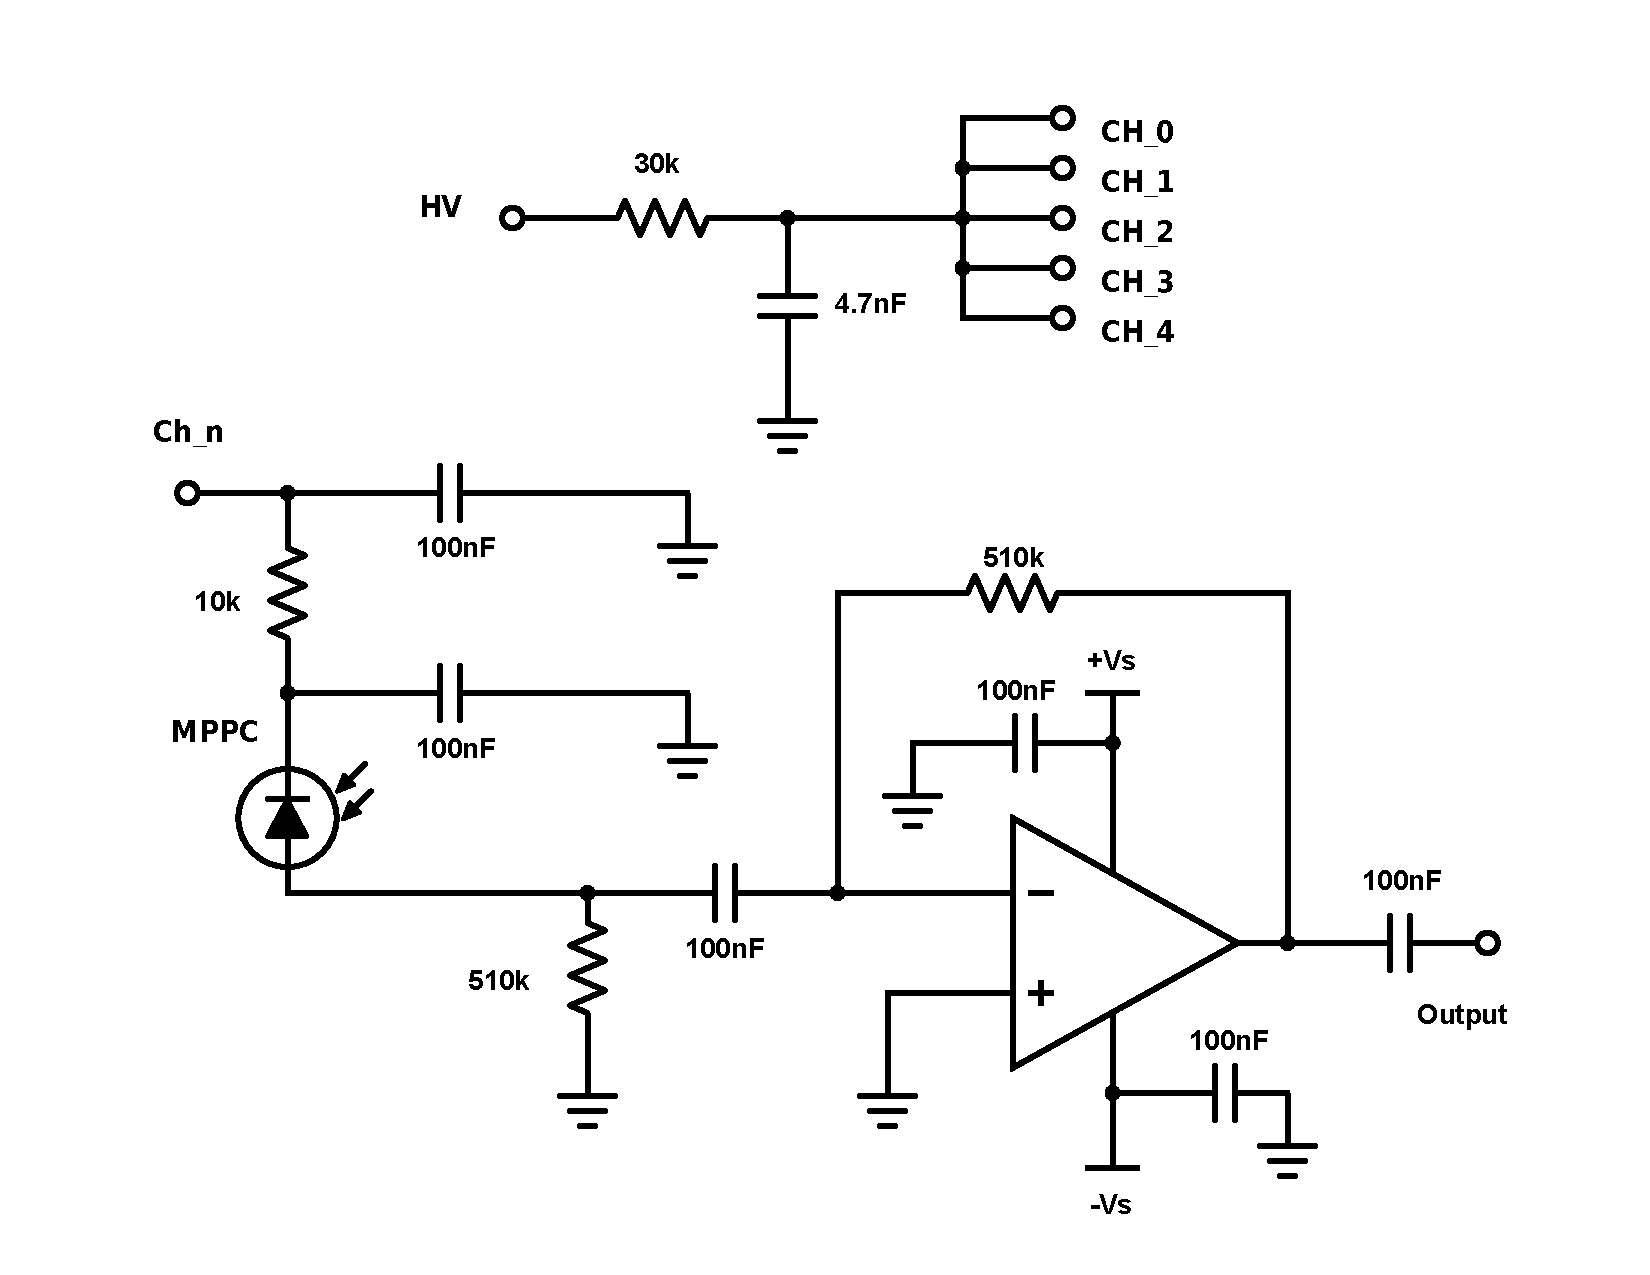
\includegraphics[width=0.5\textwidth]{circuit.pdf}
	\hspace*{\fill}
	\caption{Amplifier circuit (bottom) for each Muli-Pixel Photon Counter (MPPC). Common bias voltage for each
	mppc is shown in circuit on top.}\label{scheme}
\end{figure}

The readout consist of 50 Multi-pixel Photon Counter (MPPC) \cite{mppc}, distributed into 25 per axis. Within
each axis, 5 MPPC are grouped with similar gain to share the same bias voltage. On one axis the signal is read it from
each single MPPC, while on the other one, only two weighted signals are taken. The amplification circuit is shown in
Figure \ref{scheme}.


read-out with Wave Length Shifter (WLS) fibers. Each crystal is a Cerium doped lutetium
, a
based scintillation crystal that offers high density and a short decay time. Having similar density than BGO can offer
improvement in energy resolution, light output and better timing due to its short time decay constant (see
table \ref{property}).

\begin{table}[ht]\footnotesize
\centering
\begin{tabular*}{0.6\textwidth}{lcc}
Property & LYSO & BGO\\
\hline Density [\SI{}{g/m^3}]& 7.1 & 7.1 \\
Attenuation length for 511 keV [cm] & 1.2 & 1.0\\
Decay time [ns] & 41 & 300\\
Energy Resolution \% & 8.0 & 12.0\\
Light output, photons per keV & 32 &9 \\
Radiation Length							& 1.16 & 0.96\\
\end{tabular*}
\caption{Property comparison LYSO and BGO crystals}\label{property}
\end{table}

\section{Calibration}
\subsubsection{X-axis equalization}
{\bf Run 1459}
MIP calibration on X axis\\
\begin{figure}[ht]
	\hspace*{\fill}
	\centering
	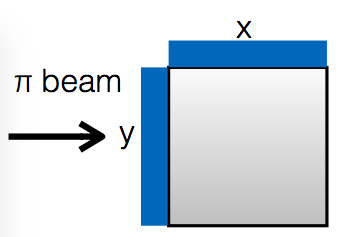
\includegraphics[width=0.5\textwidth]{mipX.png}
	\hspace*{\fill}
	\caption{}\label{mipx}
\end{figure}
Explain how the amplitude is obtained, how the pedestal are calculated.
Plot example single channel, with Vavilov pdf fit.
Plot pedestal, mean and sigma per channel.
Plot channel MIP, sigma and percentage sigma/mu per channel.

\subsubsection{Y-axis equalization}
{\bf Run 1463}
\begin{figure}[ht]
	\hspace*{\fill}
	\centering
	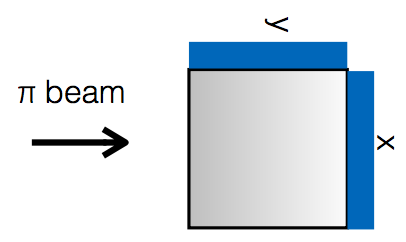
\includegraphics[width=0.5\textwidth]{mipY.png}
	\hspace*{\fill}
	\caption{}\label{mipy}
\end{figure}
Since the Y-axis has two weighted signals as readout, the readout boards must be exchanged. 
Afterwards the detector is turn over 90 degrees. Now the beam hits all the crystals along the x-axis as the scheme shows
\ref{mipy}. \par

Again the mean energy deposited on each strips it must be the energy loss by one MIP across 4mm, the width of one
crystal. 
Plot channel mip, sigma and percentage sigma/mu per channel.
\subsubsection{Z-axis configuration}
Finally the beam hits the detector as its standard configuration. The weighted signals can be correlated between each
other
{\bf Run 1467 \& Run 1468}

MIP on Z axis\\
\begin{figure}[ht]
	\hspace*{\fill}
	\centering
	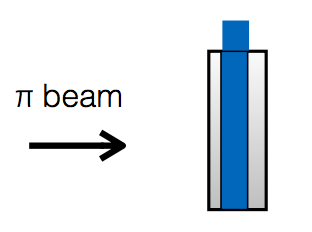
\includegraphics[width=0.5\textwidth]{mipZ.png}
	\hspace*{\fill}
	\caption{}\label{mipz}
\end{figure}


\section{Time resolution}

A time decay of about 40ns is one of the main reasons to use LYSO crystals in this experiment. With the same density as
BGO can provide faster response, therefore, a better timing.\par

To calculate the time resolution within the experiment, a time reference is provide by S1, the first detector
in front of the beam which provide the trigger for the experiment. 
Time is defined respect to the first counter S1, and calculated with constant fraction method where:....\\
The temporal resolution on a single channel is shown in ..\\
\begin{figure}[ht]
	\hspace*{\fill}
	\centering
	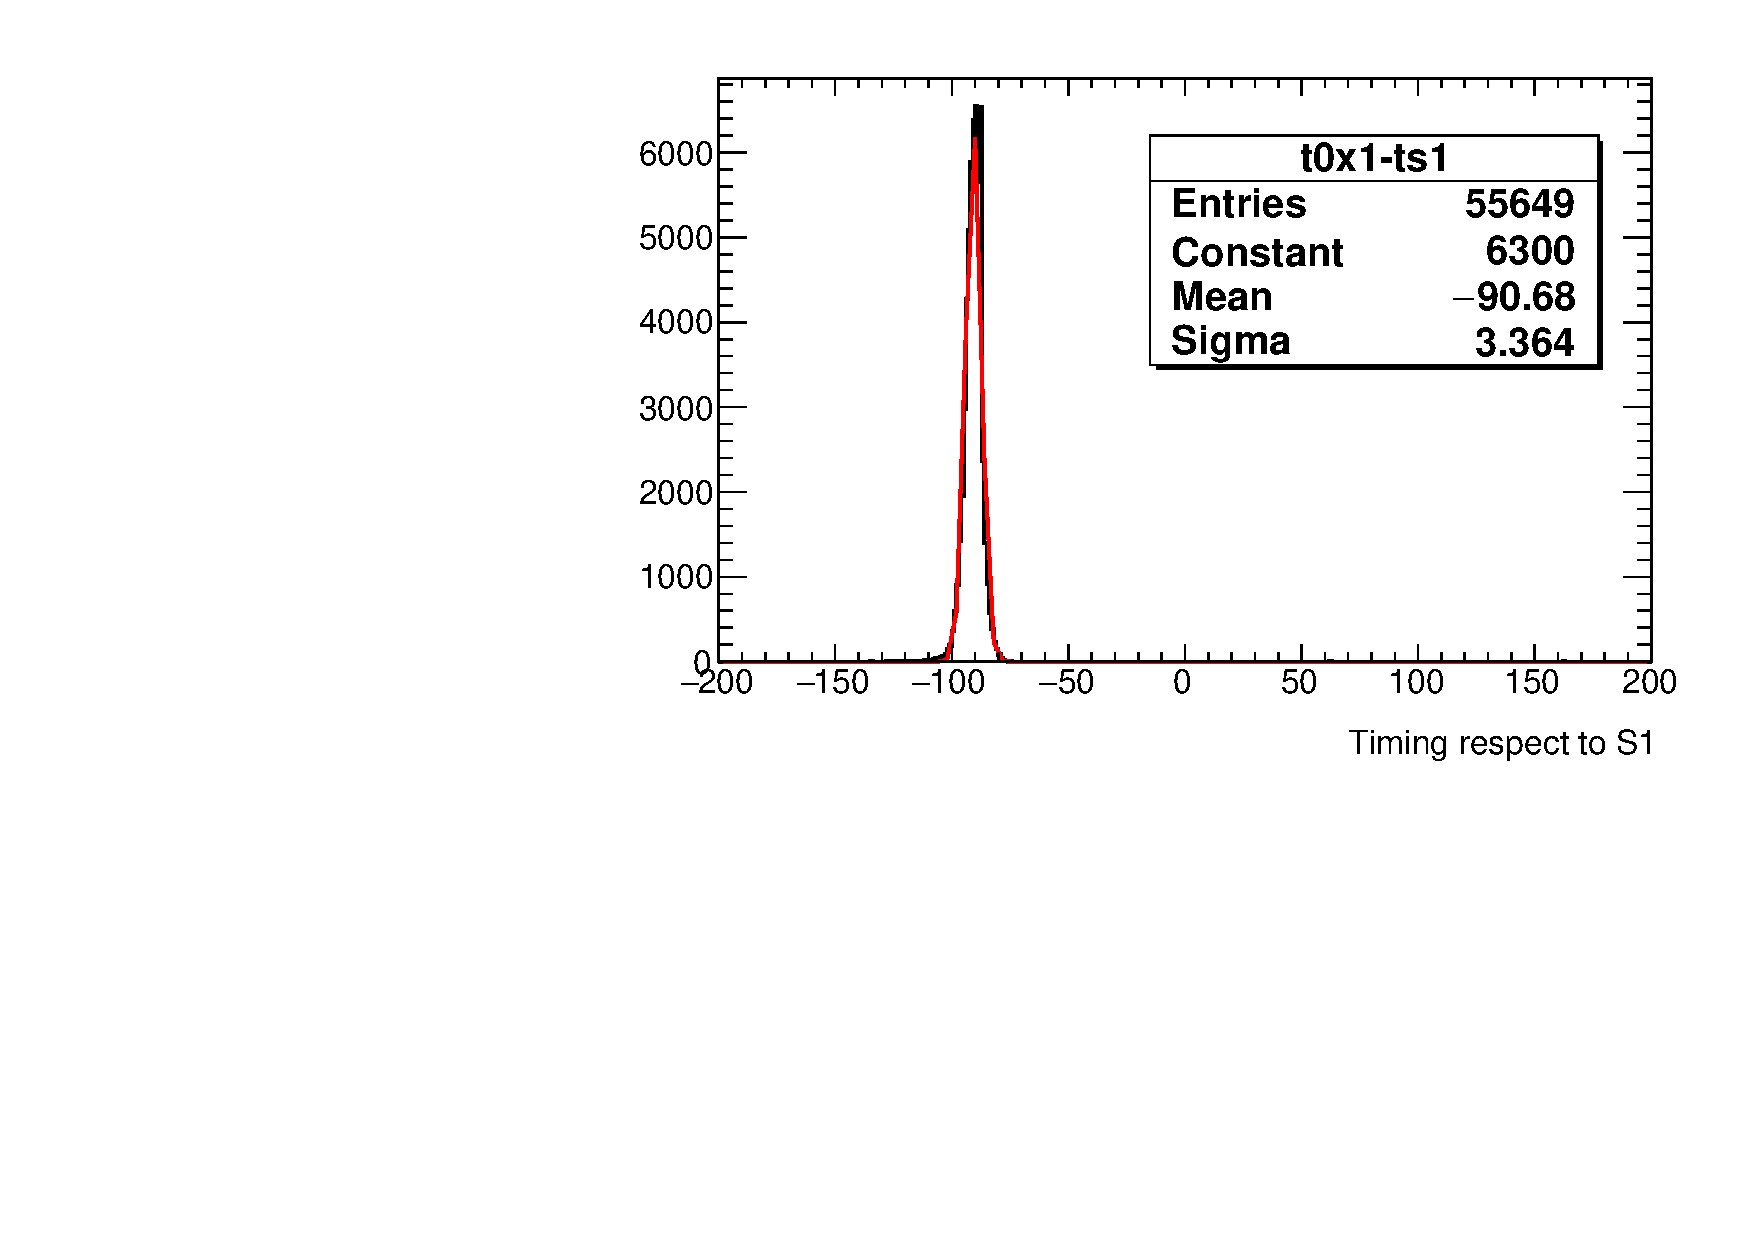
\includegraphics[width=0.5\textwidth]{ts0ts1.pdf}
	\hspace*{\fill}
	\caption{}\label{}
\end{figure}


\section{Hadron rejection}

During the July Run for the NA64 experiment, a set of runs with the LYSO detector as SRD were taken. With an average
beam intensity of 7.5$\cdot 10^5$ events/s registered on S0, these runs are considered low intensity. For tagging the
electrons and reject the hadrons, it is important to know their signature on LYSO. For this purpose, we can exploit two
features of the array of crystals.\par

Each signal from the x-axis, correspond to the amount of light produce by the column of crystals in certain x position.
All the SR produced by the electron beam in the region of the LYSO detector is collected by 25 columns. Therefore, we
should expect a homogeneous distribution of light in these 25 channels. To calculate the amount of hadrons present in
each spill or in the total triggered events, we use the electron (ECAL) and hadron (HCAL) calorimeters to provide the
identification for our analysis.\par

The next two sections show the two equivalent approach for this detector, to calculate the level of hadron suppression
factor. 
\subsection{Total energy}
In the Section \ref{bgoanal}, the level of hadron suppression is calculated using the total energy deposited as
threshold. 


\begin{figure}[ht]
	\hspace*{\fill}
	\centering
	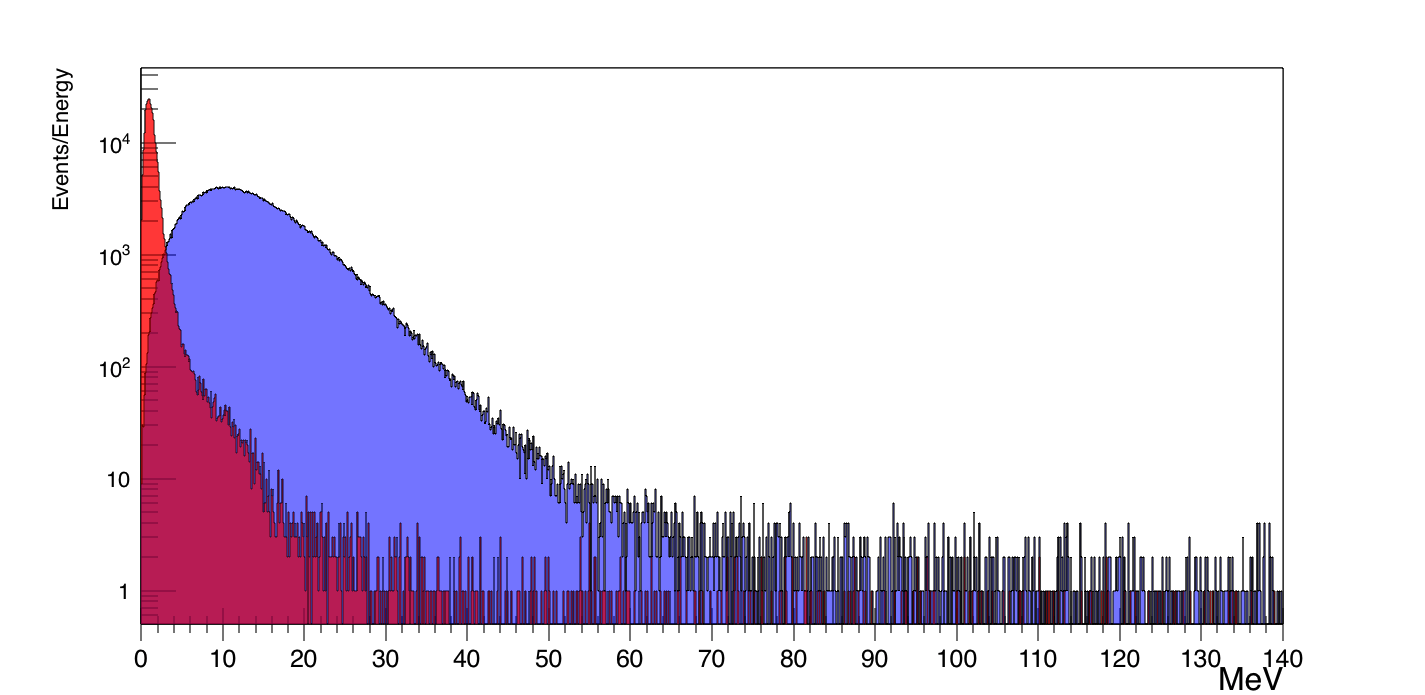
\includegraphics[width=0.9\textwidth]{srdenergy.png}
	\hspace*{\fill}
	\caption{Energy deposition of Synchrotron Radiation configuration. Electrons tagged from $S_{e^-}$ in blue and hadrons
	$S_H$ in red.}\label{srdenergy}
\end{figure}

\begin{figure}[ht]
	\hspace*{\fill}
	\centering
	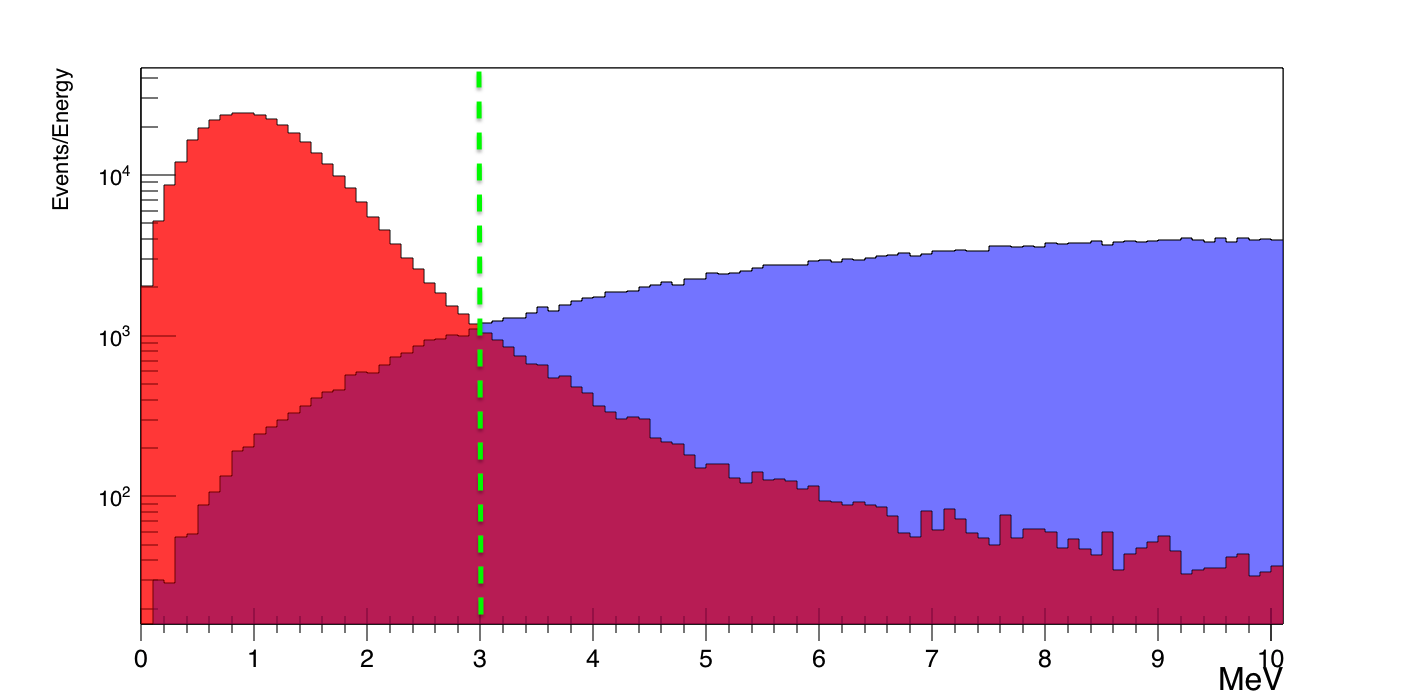
\includegraphics[width=0.7\textwidth]{srdenergyzoom.png}
	\hspace*{\fill}
	\caption{}\label{}
\end{figure}

\begin{figure}[ht]
		\centering
		\hspace*{\fill}
		\begin{subfigure}[b]{0.48\textwidth}
			\centering
			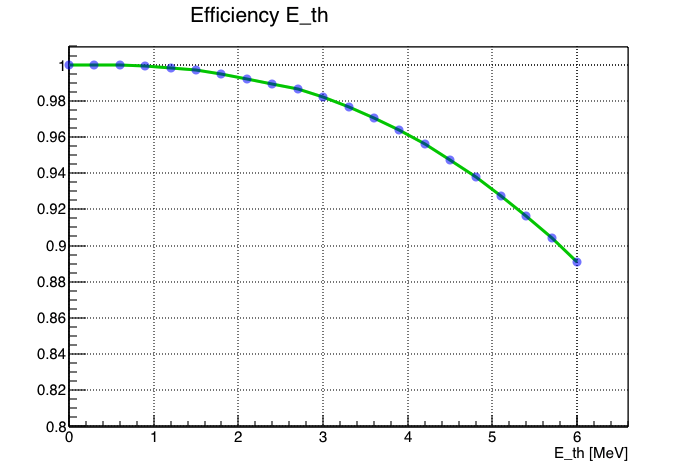
\includegraphics[width=\textwidth]{effE.png}
			\caption{}\label{}
		\end{subfigure}
		\hfill
		\begin{subfigure}[b]{0.48\textwidth}
			\centering
			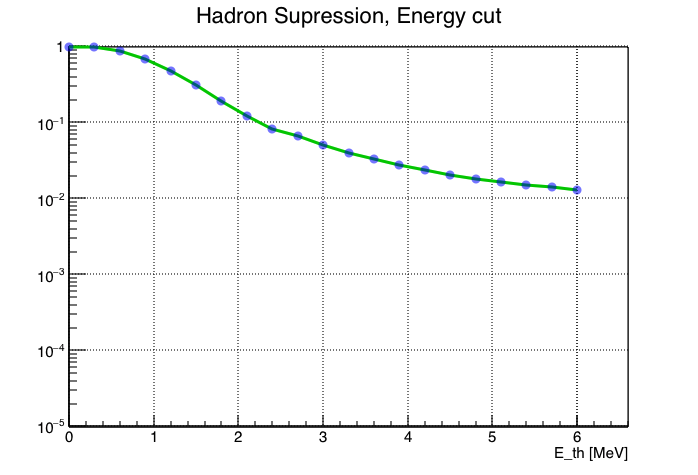
\includegraphics[width=\textwidth]{supE.png}
			\caption{}\label{}
		\end{subfigure}
		\hspace*{\fill}
		\caption{}\label{}
\end{figure}

\begin{figure}[ht]
	\hspace*{\fill}
	\centering
	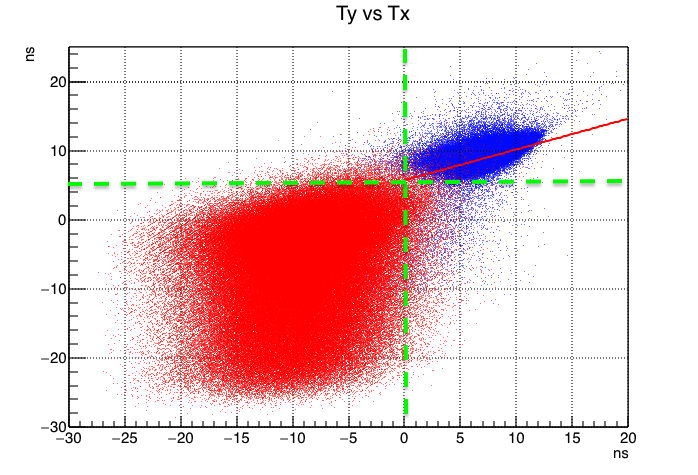
\includegraphics[width=0.8\textwidth]{tytx_fit.png}
	\hspace*{\fill}
	\caption{}\label{}
\end{figure}

\begin{figure}[ht]
		\centering
		\hspace*{\fill}
		\begin{subfigure}[b]{0.48\textwidth}
			\centering
			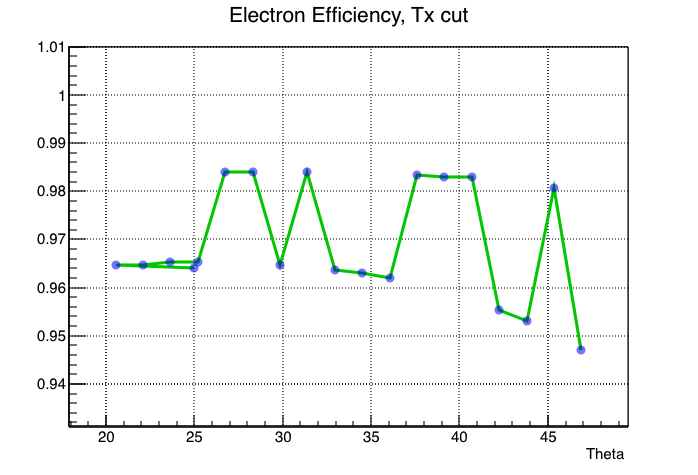
\includegraphics[width=\textwidth]{effTx.png}
			\caption{}\label{}
		\end{subfigure}
		\hfill
		\begin{subfigure}[b]{0.48\textwidth}
			\centering
			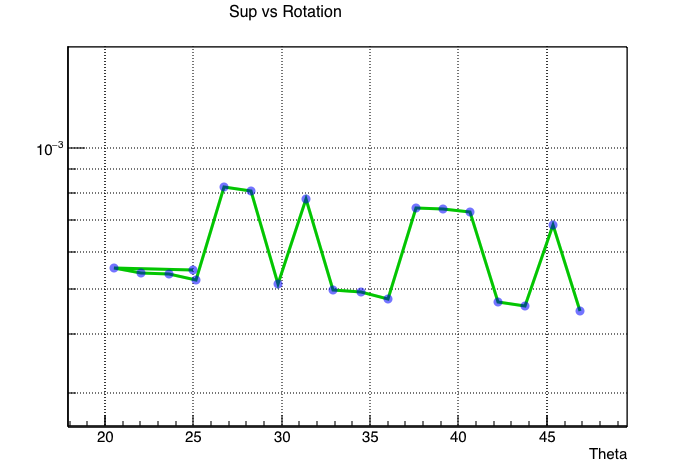
\includegraphics[width=\textwidth]{supTx.png}
			\caption{}\label{}
		\end{subfigure}
		\hspace*{\fill}
		\caption{}\label{}
\end{figure}

\begin{figure}[ht]
		\centering
		\hspace*{\fill}
		\begin{subfigure}[b]{0.48\textwidth}
			\centering
			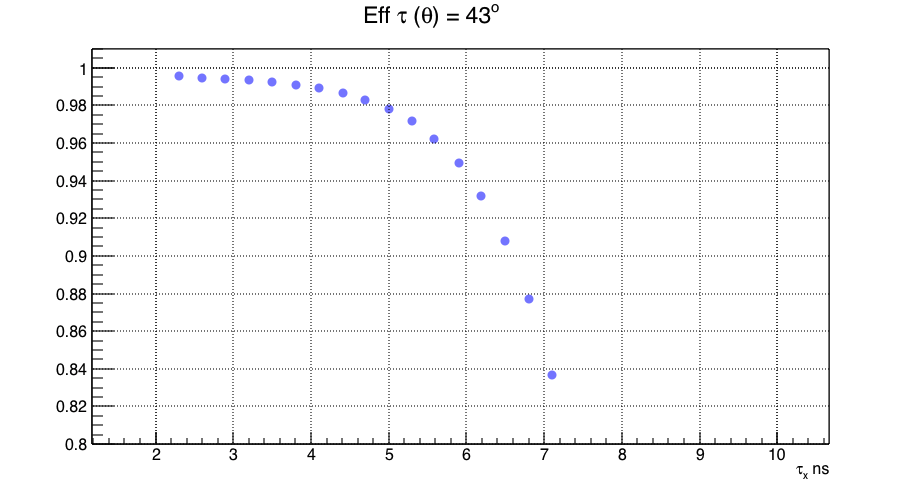
\includegraphics[width=\textwidth]{effTau.png}
			\caption{}\label{}
		\end{subfigure}
		\hfill
		\begin{subfigure}[b]{0.48\textwidth}
			\centering
			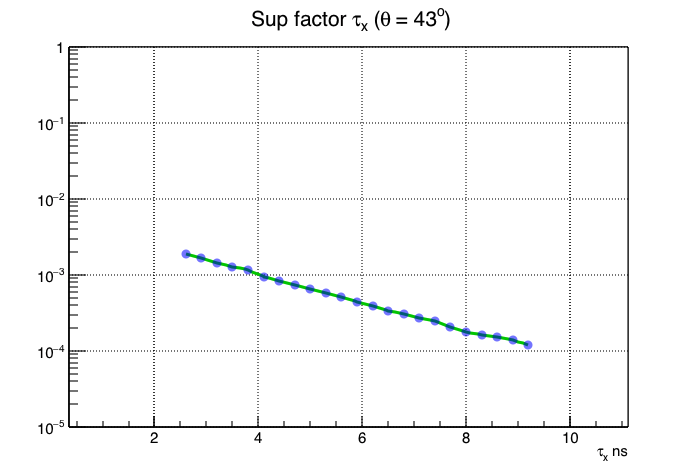
\includegraphics[width=\textwidth]{supTau.png}
			\caption{}\label{}
		\end{subfigure}
		\hspace*{\fill}
		\caption{}\label{}
\end{figure}





\subsection{Strips triggered}




\begin{figure}[ht]
	\hspace*{\fill}
	\centering
	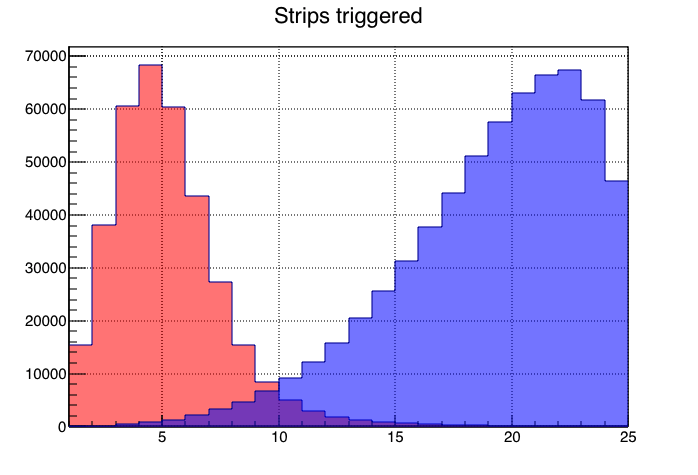
\includegraphics[width=0.7\textwidth]{stripsE.png}
	\hspace*{\fill}
	\caption{}\label{}
\end{figure}


\begin{figure}[ht]
		\centering
		\hspace*{\fill}
		\begin{subfigure}[b]{0.48\textwidth}
			\centering
			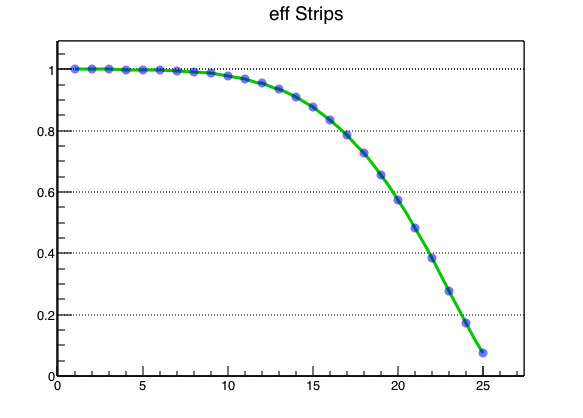
\includegraphics[width=\textwidth]{effS.png}
			\caption{}\label{}
		\end{subfigure}
		\hfill
		\begin{subfigure}[b]{0.48\textwidth}
			\centering
			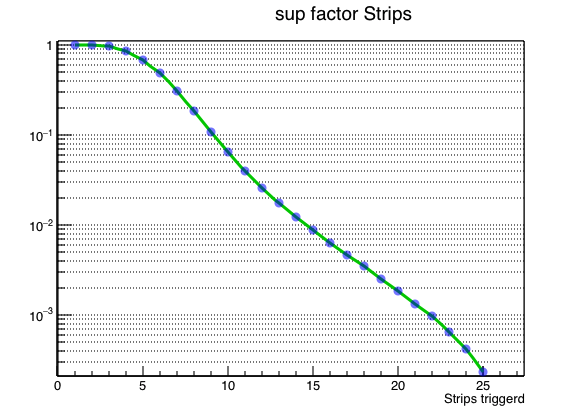
\includegraphics[width=\textwidth]{supS.png}
			\caption{}\label{}
		\end{subfigure}
		\hspace*{\fill}
		\caption{}\label{}
\end{figure}




\section{Experimental Results}

\section{Summary}


